\documentclass[border=14pt]{standalone}
\usepackage{tikz}
\usetikzlibrary{shapes.geometric, arrows.meta, positioning, fit, calc, backgrounds}
\usepackage[T1]{fontenc}
\usepackage{helvet}
\renewcommand{\familydefault}{\sfdefault}

\definecolor{cfgbg}{RGB}{236,240,241}
\definecolor{databg}{RGB}{214,234,248}
\definecolor{databorder}{RGB}{52,152,219}
\definecolor{modelbg}{RGB}{213,245,227}
\definecolor{modelborder}{RGB}{39,174,96}
\definecolor{outbg}{RGB}{253,235,208}
\definecolor{outborder}{RGB}{230,126,34}
\definecolor{hdblue}{RGB}{52,152,219}
\definecolor{hdgreen}{RGB}{39,174,96}
\definecolor{arrowcol}{RGB}{80,80,80}

\tikzset{
  stepbox/.style={
    rectangle, rounded corners=4pt, draw=#1, fill=#1!20,
    minimum width=4.8cm, minimum height=1.0cm,
    text centered, font=\small\sffamily, text width=4.6cm,
    inner sep=5pt
  },
  cfgbox/.style={
    rectangle, rounded corners=4pt, draw=black!40, fill=cfgbg,
    minimum width=11.4cm, minimum height=1.0cm,
    text centered, font=\small\sffamily, text width=11.2cm,
    inner sep=5pt
  },
  outbox/.style={
    rectangle, rounded corners=4pt, draw=outborder, fill=outbg,
    minimum width=11.4cm, minimum height=1.0cm,
    text centered, font=\small\sffamily, text width=11.2cm,
    inner sep=5pt
  },
  zonelabel/.style={
    rectangle, rounded corners=3pt, fill=#1,
    text=white, font=\small\bfseries\sffamily,
    inner sep=4pt, minimum height=0.55cm, minimum width=4.8cm,
    text centered
  },
  arr/.style={->, >=Stealth, thick, color=arrowcol},
  crossarr/.style={->, >=Stealth, thick, color=arrowcol, dashed},
}

\begin{document}
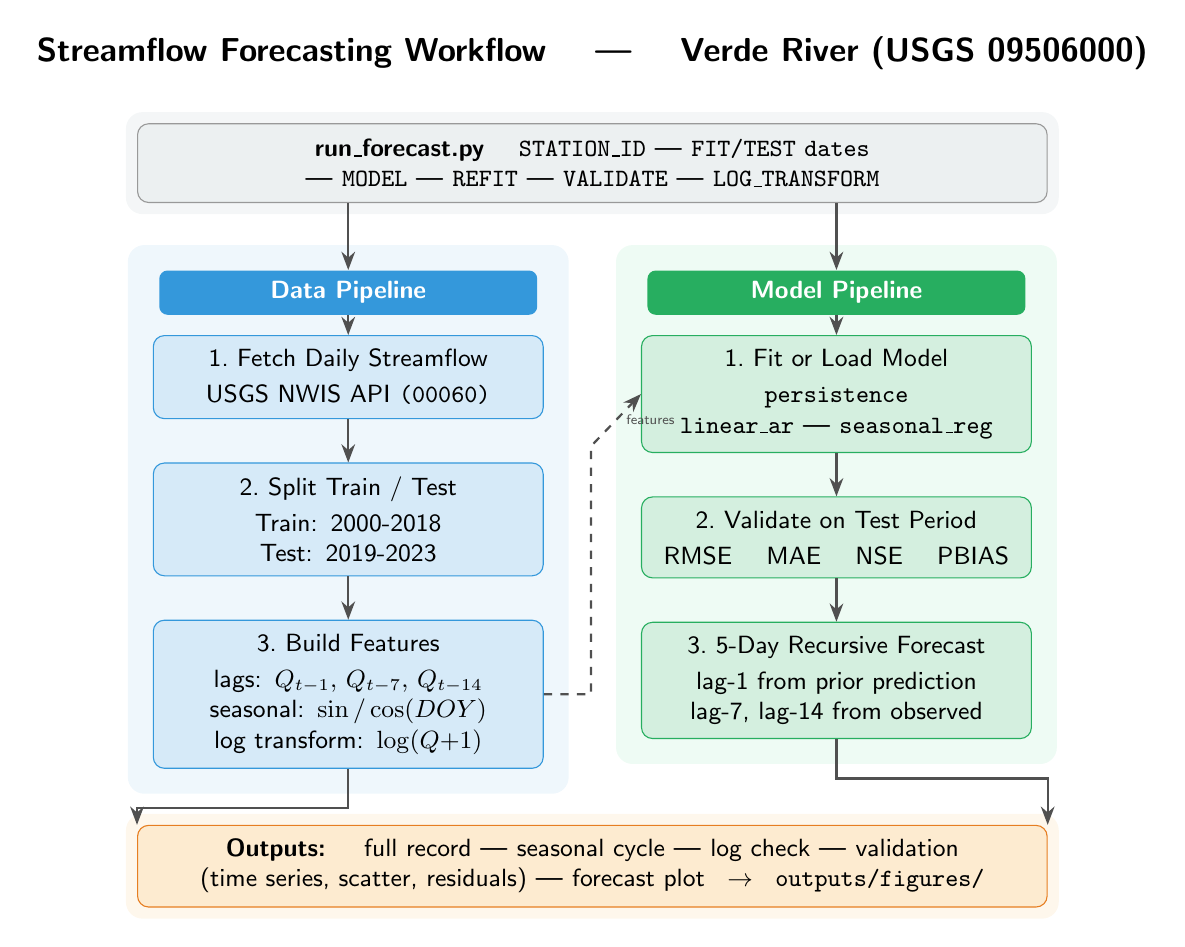
\begin{tikzpicture}[node distance=0.55cm]

%% TITLE
\node[font=\large\bfseries\sffamily] (title)
  {Streamflow Forecasting Workflow \quad | \quad Verde River (USGS 09506000)};

%% CONFIG
\node[cfgbox, below=0.55cm of title] (cfg)
  {\textbf{run\_forecast.py} \quad
   \texttt{STATION\_ID} \textbf{|} \texttt{FIT/TEST dates} \textbf{|}
   \texttt{MODEL} \textbf{|} \texttt{REFIT} \textbf{|} \texttt{VALIDATE} \textbf{|}
   \texttt{LOG\_TRANSFORM}};

%% ZONE HEADER LABELS
\node[zonelabel=hdblue, below=0.85cm of cfg, xshift=-3.1cm] (lbl_data)
  {Data Pipeline};
\node[zonelabel=hdgreen, below=0.85cm of cfg, xshift=3.1cm] (lbl_model)
  {Model Pipeline};

%% DATA COLUMN -- 3 steps
\node[stepbox=databorder, below=0.25cm of lbl_data] (fetch)
  {1.\ Fetch Daily Streamflow\\[2pt]
   USGS NWIS API \texttt{(00060)}};

\node[stepbox=databorder, below=0.55cm of fetch] (split)
  {2.\ Split Train / Test\\[2pt]
   Train: 2000-2018 \quad Test: 2019-2023};

\node[stepbox=databorder, below=0.55cm of split] (feat)
  {3.\ Build Features\\[2pt]
   lags: $Q_{t-1},\,Q_{t-7},\,Q_{t-14}$\\
   seasonal: $\sin/\cos(\text{DOY})$\\
   log transform: $\log(Q{+}1)$};

%% MODEL COLUMN -- 3 steps
\node[stepbox=modelborder, below=0.25cm of lbl_model] (fit)
  {1.\ Fit or Load Model\\[2pt]
   \texttt{persistence}\\
   \texttt{linear\_ar} \textbf{|} \texttt{seasonal\_reg}};

\node[stepbox=modelborder, below=0.55cm of fit] (val)
  {2.\ Validate on Test Period\\[2pt]
   RMSE \quad MAE \quad NSE \quad PBIAS};

\node[stepbox=modelborder, below=0.55cm of val] (fcast)
  {3.\ 5-Day Recursive Forecast\\[2pt]
   lag-1 from prior prediction\\
   lag-7, lag-14 from observed};

%% OUTPUT ROW -- anchored to midpoint of feat and fcast bottoms
\coordinate (leftbot)  at (feat.south);
\coordinate (rightbot) at (fcast.south);
\coordinate (midbot)   at ($(leftbot)!0.5!(rightbot)$);

\node[outbox, below=0.9cm of midbot] (out)
  {\textbf{Outputs:} \quad
   full record \textbf{|} seasonal cycle \textbf{|} log check \textbf{|}
   validation (time series, scatter, residuals) \textbf{|} forecast plot
   $\;\to\;$ \texttt{outputs/figures/}};

%% ARROWS -- config straight down into each zone header
\draw[arr] ([xshift=-3.1cm]cfg.south) -- (lbl_data.north);
\draw[arr] ([xshift= 3.1cm]cfg.south) -- (lbl_model.north);
\draw[arr] (lbl_data)  -- (fetch);
\draw[arr] (lbl_model) -- (fit);

%% ARROWS -- data column
\draw[arr] (fetch) -- (split);
\draw[arr] (split) -- (feat);

%% ARROWS -- model column
\draw[arr] (fit) -- (val);
\draw[arr] (val) -- (fcast);

%% CROSS ARROW -- features feed into model (routed outside both zones)
\draw[crossarr] (feat.east) -- ++(0.6,0) -- ++(0,3.15) -- (fit.west)
  node[midway, right, font=\tiny\sffamily, color=arrowcol] {features};

%% OUTPUT ARROWS -- straight down from each column
\draw[arr] (feat.south)  -- ++(0,-0.5) -| (out.north west);
\draw[arr] (fcast.south) -- ++(0,-0.5) -| (out.north east);

%% ZONE BACKGROUNDS
\begin{scope}[on background layer]
  \node[fill=databg, rounded corners=6pt, opacity=0.4,
        fit=(lbl_data)(fetch)(split)(feat), inner sep=9pt] {};
  \node[fill=modelbg, rounded corners=6pt, opacity=0.4,
        fit=(lbl_model)(fit)(val)(fcast), inner sep=9pt] {};
  \node[fill=cfgbg, rounded corners=6pt, opacity=0.6,
        fit=(cfg), inner sep=4pt] {};
  \node[fill=outbg, rounded corners=6pt, opacity=0.4,
        fit=(out), inner sep=4pt] {};
\end{scope}

\end{tikzpicture}
\end{document}
